\chapter{指標の評価}


% \newcommand{\ctext}[1]{\textcircled{\scriptsize #1}}
%丸囲み数字

\label{chap:experiment}

\section{目的}
提案する指標が,既存のサービスの推薦と比べて,より穴場である可能性が高い店を推薦することができているかを確認するため,評価を行った.

\section{使用する来店履歴データ}
高松市内の飲食店に対しての指標値を計算するため,
高松市における2020年7月28日から2020年12月24日までに呟かれた位置情報共有サービスSwarmのチェックインに連携したツイートをTwitter社の提供するSearch APIを用いて収集した.収集した10055件のチェックイン連携ツイートのうち,飲食店へのチェックインである2287件から得られた来店履歴を用いて高松市内の飲食店に対して各指標値を計算した.チェックイン先が飲食店であるかどうかは,インターネット検索により店舗が飲食店に該当するかを調べて判断した.ただし,飲食店とは,日本標準産業分類による定義\cite{restaurant}に従い,「主として注文により直ちにその場所で料理、その他の食料品または飲料を飲食させる事業所」を指す.テイクアウト専門店やスーパーマーケットなどは食料品を提供するが,本実験においては飲食店とは見なさない.また,複数の飲食店により構成されるフードコートなどの施設は飲食店とは見なさない.\par
得られた来店履歴データより,高松市において,
飲食店へチェックインしたユーザは842人,
チェックインされた飲食店は597軒,
チェックインされた全飲食店の平均延べ来店者数は3.85人であった.

\section{評価方法}
提案する各指標値が高い飲食店上位10軒,および,既存の飲食店推薦サービスである食べログ上の点数ランキング機能における2021年1月19日時点の高松市のランキング上位10軒からなる飲食店群に対して,後述するアンケートを用いて,飲食店の良質さと知名度を調査した.
ただし,高級店に日常的に通うとは考えにくく,提案する指標の利用目的に合致しないことが明らかであるため,食べログ上の,ランチとディナーの予算のうち安価な方が5000円を超えるような飲食店は推薦結果から除外したうえで,各推薦方法による上位10軒の飲食店を選んだ.
	% \subsection{推薦された飲食店の食べログ上の指標の調査}\label{exp:scrutiny}
    %
	% 	上述の飲食店群に含まれる飲食店に対して食べログ上の指標値である,点数と口コミの数とブックマークの数を調べた.また,推薦基準ごとに食べログ上の指標値の平均を求めた.

% \subsection{アンケート内容}\label{exp:questionnaire}
\section{アンケート内容}\label{exp:questionnaire}

高松市在住の男子高専生8人に対して,図\ref{fig:questionnaire}に示すアンケート用Webページを配布し,次の七項目について質問した.
	\begin{itemize}
		\item 今まで行ったことがない飲食店に積極的に行ってみたいと思うか
		\item 穴場に注目した飲食店推薦サービスがあったら利用したいと思うか
		\item 外食の頻度
	\end{itemize}
	提案指標,および,食べログ上のランキングによって推薦された各飲食店について,
	\begin{itemize}
		\item 飲食店の知名度
		\item 飲食店の料理のクオリティ
		\item 飲食店のコストパフォーマンス
		\item 飲食店に行きたいと思うか
	\end{itemize}
	ただし,外食の頻度,飲食店の知名度,飲食店の料理のクオリティ,飲食店のコストパフォーマンス,飲食店に行きたいと思うかについては,四段階から選ぶ形で尋ねた.なお,アンケート対象者にはWebページを使って飲食店のメニューの画像,および,料理の写真2枚を提示している.

	\begin{figure}[H]
		\centering
		\fbox{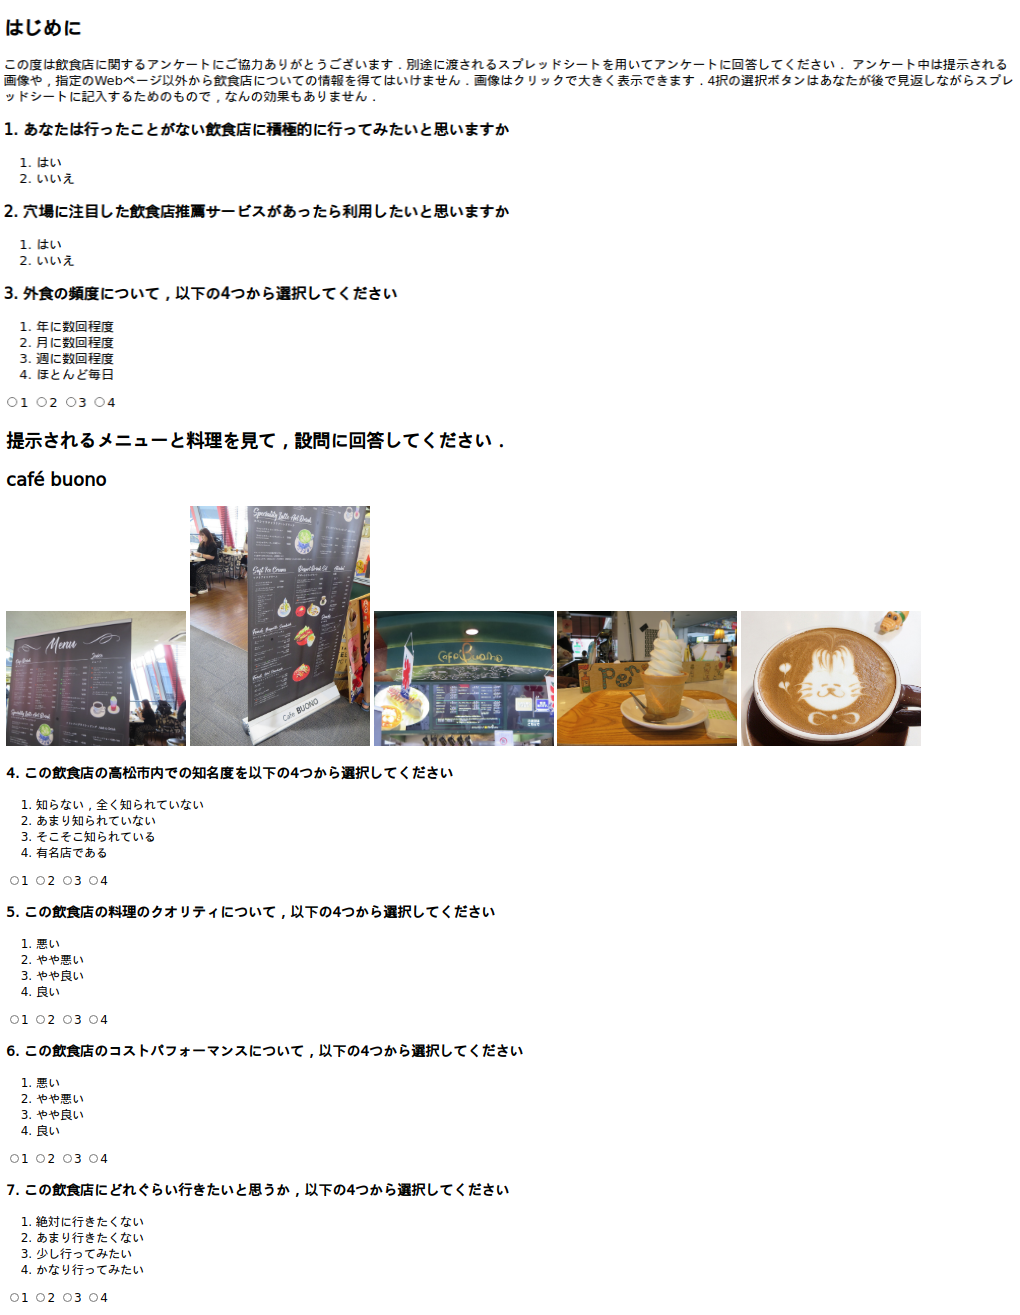
\includegraphics[width=\linewidth]{./figure/questionnaire.png}}
		\caption{アンケート用Webページ(一部)\label{fig:questionnaire}}
	\end{figure}
	\newpage
	% ただし,本実験では,飲食店の良質さが料理のクオリティ,およびコストパフォーマンスのふたつの要素から決定されると仮定した.\par
% \section{結果}
	% \subsection{食べログ上の指標値の調査結果}
	% 各指標の推薦結果上位10軒,および食べログの点数ランキング上位10軒に対して,各指標値,2020年1月22日時点における食べログ上の点数,2020年1月22日時点における食べログ上の口コミ数,2020年1月22日時点における食べログ上のブックマーク数について調べ,表\ref{table:scrutiny:VN}〜\ref{table:scrutiny:rank}にまとめた.表内の飲食店は推薦順位が高い順に並べている.また,食べログ上の点数,食べログ上の口コミ数,食べログ上のブックマーク数について,推薦方法ごとに平均値を計算し,表\ref{table:scrutiny:average}にまとめた.
	% % Please add the following required packages to your document preamble:
% \usepackage{multirow}
\begin{table}[H]
\centering
\caption{来店者新規度による推薦結果上位10軒}
\label{table:scrutiny:VN}
\small
\begin{tabular}{|c|r|r|r|r|r|r|}
\hline
\multirow{2}{*}{店名} & \multicolumn{3}{c|}{提案指標} & \multicolumn{3}{c|}{食べログ上の指標} \\ \cline{2-7}
 & \multicolumn{1}{c|}{来店者新規度} & \multicolumn{1}{c|}{やみつき度} & \multicolumn{1}{c|}{万人受け度} & \multicolumn{1}{c|}{点数} & \multicolumn{1}{c|}{口コミ数} & \multicolumn{1}{c|}{ブックマーク数} \\ \hline
炭火焼鳥 満天 & 0.143 & 3.513 & 1.000 & 3.07 & 4 & 79 \\ \hline
上海小籠包 & 0.200 & 2.342 & 1.000 & なし & なし & なし \\ \hline
つばめ家 & 0.200 & 2.342 & 1.000 & 3.30 & 11 & 427 \\ \hline
炭焼やき鳥 三吉 & 0.250 & 1.756 & 1.000 & 3.03 & 1 & 40 \\ \hline
武内食堂 鍛冶屋町店 & 0.250 & 1.756 & 1.000 & 3.08 & 4 & 94 \\ \hline
ヨコクラうどん & 0.250 & 3.212 & 0.875 & 3.62 & 54 & 1339 \\ \hline
ときわ食堂 & 0.250 & 1.756 & 1.000 & 3.00 & 4 & 38 \\ \hline
うどん市場 めんくい & 0.250 & 1.756 & 1.000 & 3.51 & 26 & 927 \\ \hline
Café Buono & 0.250 & 1.756 & 1.000 & 3.27 & 31 & 290 \\ \hline
Amazon & 0.250 & 4.792 & 0.833 & 3.15 & 6 & 96 \\ \hline
\end{tabular}
\end{table}

	% % Please add the following required packages to your document preamble:
% \usepackage{multirow}
\begin{table}[H]
\centering
\caption{やみつき度による推薦結果上位10軒}
\label{table:scrutiny:addictivity}
\small
\begin{tabular}{|c|r|r|r|r|r|r|}
\hline
\multirow{2}{*}{店名} & \multicolumn{3}{c|}{提案指標} & \multicolumn{3}{c|}{食べログ上の指標} \\ \cline{2-7}
 & \multicolumn{1}{c|}{来店者新規度} & \multicolumn{1}{c|}{やみつき度} & \multicolumn{1}{c|}{万人受け度} & \multicolumn{1}{c|}{点数} & \multicolumn{1}{c|}{口コミ数} & \multicolumn{1}{c|}{ブックマーク数} \\ \hline
ホープ軒 福岡店 & 0.333 & 5.156 & 0.733 & 3.36 & 45 & 840 \\ \hline
手打十段 うどんバカ一代 & 0.890 & 4.887 & 2.684 & 3.79 & 1034 & 38204 \\ \hline
Amazon & 0.250 & 4.792 & 0.833 & 3.15 & 6 & 96 \\ \hline
OTTIMO イオンモール高松 & 0.560 & 3.538 & 2.880 & 3.04 & 3 & 24 \\ \hline
炭火焼鳥 満天 & 0.143 & 3.513 & 1.000 & 3.07 & 4 & 79 \\ \hline
ヨコクラうどん & 0.250 & 3.212 & 0.875 & 3.62 & 54 & 1339 \\ \hline
朔日 & 0.286 & 2.627 & 0.857 & 3.17 & 12 & 745 \\ \hline
手打ちうどん ますや & 0.375 & 2.451 & 0.750 & 3.67 & 44 & 2069 \\ \hline
上海小籠包 & 0.200 & 2.342 & 1.000 & なし & なし & なし \\ \hline
つばめ家 & 0.200 & 2.342 & 1.000 & 3.30 & 11 & 427 \\ \hline
\end{tabular}
\end{table}

	% % Please add the following required packages to your document preamble:
% \usepackage{multirow}
\begin{table}[H]
\centering
\caption{万人受け度による推薦結果上位10軒}
\label{table:scrutiny:acceptability}
\small
\begin{tabular}{|c|r|r|r|r|r|r|}
\hline
\multirow{2}{*}{店名} & \multicolumn{3}{c|}{提案指標} & \multicolumn{3}{c|}{食べログ上の指標} \\ \cline{2-7}
 & \multicolumn{1}{c|}{来店者新規度} & \multicolumn{1}{c|}{やみつき度} & \multicolumn{1}{c|}{万人受け度} & \multicolumn{1}{c|}{点数} & \multicolumn{1}{c|}{口コミ数} & \multicolumn{1}{c|}{ブックマーク数} \\ \hline
めりけんや 高松駅前店 & 0.842 & 1.187 & 3.789 & 3.49 & 287 & 7275 \\ \hline
OTTIMO イオンモール高松 & 0.560 & 3.538 & 2.880 & 3.04 & 3 & 24 \\ \hline
手打十段 うどんバカ一代 & 0.890 & 4.886 & 2.684 & 3.79 & 1034 & 38204 \\ \hline
すき家 高松寿町店 & 0.400 & 1.283 & 2.400 & なし & なし & なし \\ \hline
裏きせき & 0.529 & 1.503 & 2.353 & 3.37 & 21 & 686 \\ \hline
海鮮食堂 じゃこや & 0.563 & 1.139 & 2.000 & 3.51 & 76 & 2741 \\ \hline
ダントツラーメン 岡山一番店 & 0.615 & 0.941 & 1.231 & 3.28 & 34 & 696 \\ \hline
しんみょう精肉店 鍛冶屋町店 & 0.400 & 0.970 & 1.200 & 3.04 & 3 & 243 \\ \hline
吉野家 高松瓦町店 & 0.400 & 0.970 & 1.200 & なし & なし & なし \\ \hline
麺屋 がんてつ & 0.667 & 1.791 & 1.143 & 3.38 & 52 & 703 \\ \hline
\end{tabular}
\end{table}

	% % Please add the following required packages to your document preamble:
% \usepackage{multirow}
\begin{table}[H]
\centering
\caption{食べログ上の点数による推薦結果上位10軒}
\label{table:scrutiny:rank}
\small
\begin{tabular}{|c|S|S|S|S|S|S|}
\hline
\multirow{2}{*}{店名} & \multicolumn{3}{c|}{提案指標} & \multicolumn{3}{c|}{食べログ上の指標} \\ \cline{2-7}
 & \multicolumn{1}{c|}{来店者新規度} & \multicolumn{1}{c|}{やみつき度} & \multicolumn{1}{c|}{万人受け度} & \multicolumn{1}{c|}{点数} & \multicolumn{1}{c|}{口コミ数} & \multicolumn{1}{c|}{ブックマーク数} \\ \hline
瀬戸晴れ & 0.750 & 0.290 & 0.500 & 3.94 & 77 & 3685 \\ \hline
うどん 一福 & 0.882 & 0.140 & 0.235 & 3.91 & 493 & 26692 \\ \hline
手打うどん 麦蔵 & 1.000 & 0.000 & 0.333 & 3.89 & 200 & 16172 \\ \hline
手打ちうどん はりや & 1.000 & 0.000 & 0.143 & 3.87 & 178 & 8878 \\ \hline
手打ちうどん 大蔵 & 1.000 & 0.000 & 0.500 & 3.85 & 51 & 2540 \\ \hline
うどん本陣 山田家 讃岐本店 & 0.952 & 0.059 & 0.193 & 3.82 & 452 & 20482 \\ \hline
ふる里うどん & なし & なし & なし & 3.81 & 40 & 1551 \\ \hline
手打十段 うどんバカ一代 & 0.890 & 4.886 & 2.684 & 3.79 & 1034 & 38204 \\ \hline
さか枝 & 0.909 & 0.109 & 0.182 & 3.79 & 540 & 20382 \\ \hline
竹清 & 0.912 & 0.100 & 0.167 & 3.78 & 423 & 20455 \\ \hline
\end{tabular}
\end{table}

	% \begin{table}[H]
\centering
\caption{推薦基準ごとの食べログ上の指標の平均}
\label{table:scrutiny:average}
\small
\begin{tabular}{|c|S|S|S|}
\hline
推薦基準 & \multicolumn{1}{c|}{平均点数} & \multicolumn{1}{c|}{平均口コミ数} & \multicolumn{1}{c|}{平均ブックマーク数} \\ \hline
来店者新規度 & 3.226 & 15.7 & 370.0 \\ \hline
やみつき度 & 3.352 & 134.8 & 4869.2 \\ \hline
万人受け度 & 3.298 & 148.5 & 5068.6 \\ \hline
食べログ上のランキング & 3.845 & 348.8 & 15904.1 \\ \hline
\end{tabular}
\end{table}

	% \newpage

	% \subsection{アンケート結果}
	\section{アンケート結果}
	\ref{exp:questionnaire}に示した
	%各指標の推薦結果上位10軒,および食べログの点数ランキング上位10軒に対しての
	アンケートの結果を,表\ref{table:questionnaire:tendency}〜\ref{table:questionnaire:rank}にまとめた.表内の飲食店は推薦順位が高い順に並べている.また,各推薦方法,および,各項目に対し「低い/絶対に行きたくない」または「やや低い/あまり行きたくない」と評価された数と「やや高い/少し行ってみたい」または「高い/かなり行ってみたい」と評価された数を表\ref{table:questionnaire:sum}にまとめた.
	\begin{table}[H]
\centering
\caption{外食の傾向についてのアンケート結果}
\label{table:questionnaire:tendency}
\small
\scalebox{0.7}[1.0]{
\begin{tabular}{|l|l|l|}
\hline
項目 & はい & いいえ \\ \hline
行ったことない店に行きたいか & 4 & 4 \\ \hline
穴場飲食店推薦サービスを利用したいか & 6 & 2 \\ \hline
\end{tabular}
}
\end{table}

	\begin{table}[H]
\centering
\caption{外食の傾向についてのアンケート結果}
\label{table:questionnaire:frequency}
\small
\begin{tabular}{|c|r|r|r|r|}
\hline
項目 & 年に数回 & 月に数回 & 週に数回 & ほぼ毎日 \\ \hline
外食の頻度 & 1 & 6 & 1 & 0 \\ \hline
\end{tabular}
\end{table}

	% Please add the following required packages to your document preamble:
% \usepackage{multirow}
\begin{table}[H]
\centering
\caption{来店者新規度による推薦のアンケート結果抜粋}
\label{table:questionnaire:VN}
\small
\scalebox{0.7}[1.0]{
\begin{tabular}{|l|l|l|l|l|l|}
\hline
店名 & 項目 & 低い/絶対に行きたくない & やや低い/あまり行きたくない & やや高い/少し行ってみたい & 高い/かなり行ってみたい \\ \hline
\multirow{4}{*}{炭火焼鳥 満天} & 知名度 & 5 & 1 & 1 & 1 \\ \cline{2-6}
 & 料理のクオリティ & 0 & 1 & 3 & 4 \\ \cline{2-6}
 & コストパフォーマンス & 0 & 4 & 4 & 0 \\ \cline{2-6}
 & 行きたいと思うか & 1 & 1 & 3 & 3 \\ \hline
\multirow{4}{*}{上海小籠包} & 知名度 & 4 & 2 & 2 & 0 \\ \cline{2-6}
 & 料理のクオリティ & 0 & 0 & 3 & 5 \\ \cline{2-6}
 & コストパフォーマンス & 0 & 0 & 5 & 3 \\ \cline{2-6}
 & 行きたいと思うか & 0 & 0 & 4 & 4 \\ \hline
\multirow{4}{*}{つばめ家} & 知名度 & 6 & 0 & 2 & 0 \\ \cline{2-6}
 & 料理のクオリティ & 0 & 1 & 3 & 4 \\ \cline{2-6}
 & コストパフォーマンス & 1 & 3 & 3 & 1 \\ \cline{2-6}
 & 行きたいと思うか & 0 & 4 & 3 & 1 \\ \hline
\end{tabular}
}
\end{table}

	% Please add the following required packages to your document preamble:
% \usepackage{multirow}
\begin{table}[H]
\centering
\caption{やみつき度による推薦のアンケート結果}
\label{table:questionnaire:addictivity}
\small
\begin{tabular}{|c|c|r|r|r|r|}
\hline
店名 & 項目 & \multicolumn{1}{Wc{4em}|}{低い} & \multicolumn{1}{Wc{4em}|}{やや低い} & \multicolumn{1}{Wc{4em}|}{やや高い} & \multicolumn{1}{Wc{4em}|}{高い} \\ \hline
\multirow{4}{*}{\begin{tabular}[c]{@{}c@{}}ホープ軒 \\ 福岡店\end{tabular}} & 知名度 & 3 & 1 & 2 & 2 \\ \cline{2-6} 
 & 料理のクオリティ & 0 & 1 & 4 & 3 \\ \cline{2-6} 
 & コストパフォーマンス & 1 & 3 & 3 & 1 \\ \cline{2-6} 
 & 行きたいと思うか & 0 & 2 & 4 & 2 \\ \hline
\multirow{4}{*}{\begin{tabular}[c]{@{}c@{}}手打十段 \\ うどんバカ一代\end{tabular}} & 知名度 & 3 & 1 & 1 & 3 \\ \cline{2-6} 
 & 料理のクオリティ & 0 & 0 & 5 & 3 \\ \cline{2-6} 
 & コストパフォーマンス & 0 & 1 & 7 & 0 \\ \cline{2-6} 
 & 行きたいと思うか & 0 & 1 & 5 & 2 \\ \hline
\multirow{4}{*}{Amazon} & 知名度 & 7 & 1 & 0 & 0 \\ \cline{2-6} 
 & 料理のクオリティ & 2 & 2 & 4 & 0 \\ \cline{2-6} 
 & コストパフォーマンス & 2 & 1 & 4 & 1 \\ \cline{2-6} 
 & 行きたいと思うか & 2 & 6 & 0 & 0 \\ \hline
\multirow{4}{*}{\begin{tabular}[c]{@{}c@{}}OTTIMO \\ イオンモール高松\end{tabular}} & 知名度 & 4 & 3 & 1 & 0 \\ \cline{2-6} 
 & 料理のクオリティ & 0 & 0 & 6 & 2 \\ \cline{2-6} 
 & コストパフォーマンス & 0 & 3 & 5 & 0 \\ \cline{2-6} 
 & 行きたいと思うか & 0 & 2 & 5 & 1 \\ \hline
\multirow{4}{*}{\begin{tabular}[c]{@{}c@{}}炭火焼鳥 \\ 満天\end{tabular}} & 知名度 & 5 & 1 & 1 & 1 \\ \cline{2-6} 
 & 料理のクオリティ & 0 & 1 & 3 & 4 \\ \cline{2-6} 
 & コストパフォーマンス & 0 & 4 & 4 & 0 \\ \cline{2-6} 
 & 行きたいと思うか & 1 & 1 & 3 & 3 \\ \hline
\multirow{4}{*}{ヨコクラうどん} & 知名度 & 5 & 1 & 2 & 0 \\ \cline{2-6} 
 & 料理のクオリティ & 0 & 1 & 6 & 1 \\ \cline{2-6} 
 & コストパフォーマンス & 0 & 1 & 4 & 3 \\ \cline{2-6} 
 & 行きたいと思うか & 0 & 2 & 4 & 2 \\ \hline
\multirow{4}{*}{朔日} & 知名度 & 7 & 0 & 1 & 0 \\ \cline{2-6} 
 & 料理のクオリティ & 0 & 1 & 3 & 4 \\ \cline{2-6} 
 & コストパフォーマンス & 1 & 2 & 4 & 1 \\ \cline{2-6} 
 & 行きたいと思うか & 0 & 1 & 6 & 1 \\ \hline
\multirow{4}{*}{\begin{tabular}[c]{@{}c@{}}手打ちうどん \\ ますや\end{tabular}} & 知名度 & 4 & 2 & 1 & 1 \\ \cline{2-6} 
 & 料理のクオリティ & 0 & 2 & 3 & 3 \\ \cline{2-6} 
 & コストパフォーマンス & 0 & 1 & 5 & 2 \\ \cline{2-6} 
 & 行きたいと思うか & 0 & 2 & 4 & 2 \\ \hline
\multirow{4}{*}{上海小籠包} & 知名度 & 4 & 2 & 2 & 0 \\ \cline{2-6} 
 & 料理のクオリティ & 0 & 0 & 3 & 5 \\ \cline{2-6} 
 & コストパフォーマンス & 0 & 0 & 5 & 3 \\ \cline{2-6} 
 & 行きたいと思うか & 0 & 0 & 4 & 4 \\ \hline
\multirow{4}{*}{つばめ家} & 知名度 & 6 & 0 & 2 & 0 \\ \cline{2-6} 
 & 料理のクオリティ & 0 & 1 & 3 & 4 \\ \cline{2-6} 
 & コストパフォーマンス & 1 & 3 & 3 & 1 \\ \cline{2-6} 
 & 行きたいと思うか & 0 & 4 & 3 & 1 \\ \hline
\end{tabular}
\end{table}

	% Please add the following required packages to your document preamble:
% \usepackage{multirow}
\begin{table}[H]
\centering
\caption{万人受け度による推薦のアンケート結果抜粋}
\label{table:questionnaire:acceptability}
\small
\scalebox{0.7}[1.0]{
\begin{tabular}{|l|l|l|l|l|l|}
\hline
店名 & 項目 & 低い/絶対に行きたくない & やや低い/あまり行きたくない & やや高い/少し行ってみたい & 高い/かなり行ってみたい \\ \hline
\multirow{4}{*}{めりけんや 高松駅前店} & 知名度 & 3 & 1 & 3 & 1 \\ \cline{2-6}
 & 料理のクオリティ & 0 & 3 & 4 & 1 \\ \cline{2-6}
 & コストパフォーマンス & 0 & 1 & 4 & 3 \\ \cline{2-6}
 & 行きたいと思うか & 0 & 3 & 4 & 1 \\ \hline
\multirow{4}{*}{OTTIMO イオンモール高松} & 知名度 & 4 & 3 & 1 & 0 \\ \cline{2-6}
 & 料理のクオリティ & 0 & 0 & 6 & 2 \\ \cline{2-6}
 & コストパフォーマンス & 0 & 3 & 5 & 0 \\ \cline{2-6}
 & 行きたいと思うか & 0 & 2 & 5 & 1 \\ \hline
\multirow{4}{*}{手打十段 うどんバカ一代} & 知名度 & 3 & 1 & 1 & 3 \\ \cline{2-6}
 & 料理のクオリティ & 0 & 0 & 5 & 3 \\ \cline{2-6}
 & コストパフォーマンス & 0 & 1 & 7 & 0 \\ \cline{2-6}
 & 行きたいと思うか & 0 & 1 & 5 & 2 \\ \hline
\end{tabular}
}
\end{table}

	% Please add the following required packages to your document preamble:
% \usepackage{multirow}
\begin{table}[H]
\centering
\caption{食べログ上の点数による推薦のアンケート結果}
\label{table:questionnaire:rank}
\small
\begin{tabular}{|c|c|r|r|r|r|}
\hline
店名 & 項目 & \multicolumn{1}{Wc{4em}|}{低い} & \multicolumn{1}{Wc{4em}|}{やや低い} & \multicolumn{1}{Wc{4em}|}{やや高い} & \multicolumn{1}{Wc{4em}|}{高い} \\ \hline
\multirow{4}{*}{おうどん 瀬戸晴れ} & 知名度 & 5 & 1 & 1 & 1 \\ \cline{2-6}
 & クオリティ & 0 & 0 & 2 & 6 \\ \cline{2-6}
 & コストパフォーマンス & 1 & 3 & 4 & 0 \\ \cline{2-6}
 & 行きたいと思うか & 0 & 2 & 3 & 3 \\ \hline
\multirow{4}{*}{うどん 一福} & 知名度 & 3 & 1 & 3 & 1 \\ \cline{2-6}
 & 料理のクオリティ & 0 & 1 & 5 & 2 \\ \cline{2-6}
 & コストパフォーマンス & 0 & 1 & 2 & 5 \\ \cline{2-6}
 & 行きたいと思うか & 0 & 3 & 4 & 1 \\ \hline
\multirow{4}{*}{手打うどん 麦蔵} & 知名度 & 5 & 1 & 2 & 0 \\ \cline{2-6}
 & 料理のクオリティ & 0 & 3 & 4 & 1 \\ \cline{2-6}
 & コストパフォーマンス & 2 & 5 & 1 & 0 \\ \cline{2-6}
 & 行きたいと思うか & 1 & 5 & 2 & 0 \\ \hline
\multirow{4}{*}{手打うどん はりや} & 知名度 & 4 & 1 & 3 & 0 \\ \cline{2-6}
 & 料理のクオリティ & 0 & 0 & 2 & 6 \\ \cline{2-6}
 & コストパフォーマンス & 3 & 0 & 4 & 1 \\ \cline{2-6}
 & 行きたいと思うか & 1 & 0 & 3 & 4 \\ \hline
\multirow{4}{*}{手打ちうどん大蔵} & 知名度 & 5 & 1 & 1 & 1 \\ \cline{2-6}
 & 料理のクオリティ & 0 & 0 & 1 & 7 \\ \cline{2-6}
 & コストパフォーマンス & 1 & 4 & 3 & 0 \\ \cline{2-6}
 & 行きたいと思うか & 1 & 2 & 4 & 1 \\ \hline
\multirow{4}{*}{うどん本陣 山田家} & 知名度 & 3 & 0 & 1 & 4 \\ \cline{2-6}
 & 料理のクオリティ & 1 & 0 & 0 & 7 \\ \cline{2-6}
 & コストパフォーマンス & 2 & 2 & 3 & 1 \\ \cline{2-6}
 & 行きたいと思うか & 0 & 3 & 3 & 2 \\ \hline
\multirow{4}{*}{ふる里うどん} & 知名度 & 5 & 1 & 1 & 1 \\ \cline{2-6}
 & 料理のクオリティ & 0 & 0 & 8 & 0 \\ \cline{2-6}
 & コストパフォーマンス & 0 & 3 & 4 & 1 \\ \cline{2-6}
 & 行きたいと思うか & 0 & 3 & 4 & 1 \\ \hline
\multirow{4}{*}{手打十段 うどんバカ一代} & 知名度 & 3 & 1 & 1 & 3 \\ \cline{2-6}
 & 料理のクオリティ & 0 & 0 & 5 & 3 \\ \cline{2-6}
 & コストパフォーマンス & 0 & 1 & 7 & 0 \\ \cline{2-6}
 & 行きたいと思うか & 0 & 1 & 5 & 2 \\ \hline
\multirow{4}{*}{さか枝うどん} & 知名度 & 2 & 0 & 2 & 4 \\ \cline{2-6}
 & 料理のクオリティ & 0 & 3 & 1 & 4 \\ \cline{2-6}
 & コストパフォーマンス & 0 & 2 & 1 & 5 \\ \cline{2-6}
 & 行きたいと思うか & 0 & 3 & 4 & 1 \\ \hline
\multirow{4}{*}{竹清 本店} & 知名度 & 4 & 3 & 0 & 1 \\ \cline{2-6}
 & 料理のクオリティ & 0 & 2 & 5 & 1 \\ \cline{2-6}
 & コストパフォーマンス & 0 & 1 & 2 & 5 \\ \cline{2-6}
 & 行きたいと思うか & 1 & 2 & 3 & 2 \\ \hline
\end{tabular}
\end{table}

	\begin{table}[H]
\centering
\caption{アンケート結果の合計}
\label{table:questionnaire:sum}
\small
\begin{tabular}{|c|c|r|r|}
\hline
項目 & 推薦方法 & 悪い\footnotemark[3] & 良い\footnotemark[4] \\ \hline
\multirow{4}{*}{知名度} & 来店者新規度 & 67 & 13 \\ \cline{2-4}
 & やみつき度 & 60 & 20 \\ \cline{2-4}
 & 万人受け度 & 35 & 45 \\ \cline{2-4}
 & 食べログ上の点数 & 49 & 31 \\ \hline
\multirow{4}{*}{料理のクオリティ} & 来店者新規度 & 11 & 69 \\ \cline{2-4}
 & やみつき度 & 11 & 69 \\ \cline{2-4}
 & 万人受け度 & 11 & 69 \\ \cline{2-4}
 & 食べログ上の点数 & 10 & 70 \\ \hline
\multirow{4}{*}{コストパフォーマンス} & 来店者新規度 & 24 & 56 \\ \cline{2-4}
 & やみつき度 & 24 & 56 \\ \cline{2-4}
 & 万人受け度 & 9 & 71 \\ \cline{2-4}
 & 食べログ上の点数 & 31 & 49 \\ \hline
\multirow{4}{*}{行きたいと思うか} & 来店者新規度 & 24 & 56 \\ \cline{2-4}
 & やみつき度 & 24 & 56 \\ \cline{2-4}
 & 万人受け度 & 20 & 60 \\ \cline{2-4}
 & 食べログ上の点数 & 28 & 52 \\ \hline
\end{tabular}
\end{table}
\footnotetext[3]{低い/絶対に行きたくない,またはやや低い/あまり行きたくないと評価された数}
\footnotetext[4]{やや高い/少し行ってみたい,または高い/かなり行ってみたいと評価された数}

	\par
	表\ref{table:questionnaire:tendency}から,今回のアンケート対象者のうち,半数が行ったことがない店に行きたいと考えており,穴場飲食店推薦サービスの需要があることがわかる.\par
	表\ref{table:questionnaire:frequency}から,今回のアンケート対象者の多くが月に数回の頻度で外食することがわかる.\par
	表\ref{table:questionnaire:VN}〜\ref{table:questionnaire:rank}から,来店者新規度による推薦結果のうち知名度が高いと評価されたのは一軒だけであり,他の推薦方法と比べて有名店が推薦されていないことがわかる.また,やみつき度による推薦結果のうち5軒が来店者新規度でも推薦されており,来店者新規度で推薦されなかった5軒のうち3軒が知名度が高いと評価されている.万人受け度による推薦結果は牛丼全国チェーン店が2軒含まれており,知名度が高いと評価された店は10軒のうち8軒である.さらに,食べログ上のランキングによる推薦はうどん店に偏っている.\par
	表\ref{table:questionnaire:sum}から,料理のクオリティに関しては推薦方法による差がほぼ無いことがわかる.また,コストパフォーマンスは万人受け度による推薦だけが突出して高い評価を得ており,来店者新規度とやみつき度は差がなく,食べログは少し評価が低くなっている.

\section{指標の評価}
アンケート結果から提案する指標について評価を行う.\par
% 食べログ上の点数の平均値の差から,提案指標による推薦では食べログの点数ランキングでは推薦されない飲食店を多く推薦できていることがわかる.
% \par
% また,
アンケートより,来店者新規度,および,やみつき度による推薦結果は知名度が低く,万人受け度,および,食べログ上の点数による推薦結果は知名度が高い傾向にあるといえる.料理のクオリティに関しては推薦方法によらず,同じような結果となった.
コストパフォーマンスは万人受け度による推薦だけが突出して高い評価を得ており,その他の推薦方法では同じような結果となった.%また,もっとも行きたいと思う飲食店を推薦できたのは万人受け度であった.\par
\par
よって,提案指標は食べログでは推薦されない飲食店を推薦できているが,穴場を推薦できているといえるのは来店者新規度とやみつき度の二つだけであり,もっとも穴場を推薦できているのは来店者新規度であり,万人受け度は穴場を推薦できていない.
%万人受け度が推薦する飲食店は,穴場ではないが,男子高専生が行きたいと思う飲食店であり,もっとも良質であると考えられる.
